\documentclass[../../main.tex]{subfiles}
\begin{document}
\onlyinsubfile{
\setcounter{chapter}{1}
}
\notinsubfile{}


\begin{tikzpicture}%
% On main layer:
\definecolor{lila}{RGB}{236,211,236}
\definecolor{lemonchiffon}{RGB}{255,250,205}
\fill[color=lila] (-7,-6.5) rectangle +(\the\textwidth,9.5);%vlak van tekening

%het apparaat
\begin{scope}[xshift=-4cm, yshift=-1.5cm]
   %vier kleuren lampen
  \draw [fill=red           ](-1.4,2.5) circle (.3cm);
%  \draw [fill=red!50!black  ](-1.4,2.5) circle (.3cm);
%  \draw [fill=green         ]( 1.4,2.5) circle (.3cm);
  \draw [fill=green!50!black]( 1.4,2.5) circle (.3cm);
  %extra lichtstralen
  \foreach \ray in {-20,0,20,160,180,200} \draw (-1.4,2.5)+(\ray:.4cm) -- +(\ray:0.6cm);
  %lamphouders
  \draw [fill=black](-1.5,2) rectangle (-1.3,2.2);
  \draw [fill=black]( 1.3,2) rectangle ( 1.5,2.2);
  %box
  \draw[thin, rounded corners=10pt](-2,-2)rectangle(2,2);
  \begin{scope}[yshift=-1cm]%wijzers in drie standen
    \tikzstyle{base}=[circle,draw=red!50,fill=red!50,thick]
    \node (o) at (0,0){};
    \node (a) at( 110:2.5cm)[base]{A};
    \node (v) at(  90:2.5cm)[base]{V};
    \node (b) at( +70:2.5cm)[base]{B};
    \draw[dashed] ($(o)-(0,0.)$) -- (a);
    \draw[dashed] ($(o)-(0,0.)$) -- (v);  
    \draw[dashed] ($(o)-(0,0.)$) -- (b);
    %wijzerknop
    \fill[rotate= 20] (-.12,-.5) --(.12,-.5) -- (.12,0) -- (0,1) -- (-.12,0);
    \fill[rotate=  0] (-.12,-.5) --(.12,-.5) -- (.12,0) -- (0,1) -- (-.12,0);
    \fill[rotate=-20] (-.12,-.5) --(.12,-.5) -- (.12,0) -- (0,1) -- (-.12,0);
  \end{scope}
\end{scope}

\begin{scope}[xshift=0.0cm, yshift=0.5cm, scale=.55]
  \tikzstyle{base}=[circle,draw=red!50,inner sep=0pt, fill=red!50,thick]
  \node (o) at (0,0){};
  \node (a) at( 110:2.5cm)[base]{A};
  \node (v) at(  90:2.5cm)[base]{V};
  \node (b) at( +70:2.5cm)[base]{B};
  \draw[dashed] ($(o)-(0,0.)$) -- (a);
  \draw[dashed] ($(o)-(0,0.)$) -- (v);  
  \draw[dashed] ($(o)-(0,0.)$) -- (b);
%aanwijzerknop
  \fill[rotate= 0] (-.12,-.5) --(.12,-.5) -- (.12,0) -- (0,1) -- (-.12,0);
\end{scope}

\begin{scope}[xshift=0.0cm, yshift=-2.5cm, scale=.55]
  \tikzstyle{base}=[circle,draw=red!50,inner sep=0pt, fill=red!50,thick]
  \node (o) at (0,0){};
  \node (a) at( 110:2.5cm)[base]{A};
  \node (v) at(  90:2.5cm)[base]{V};
  \node (b) at( +70:2.5cm)[base]{B};
  \draw[dashed] ($(o)-(0,0.)$) -- (a);
  \draw[dashed] ($(o)-(0,0.)$) -- (v);  
  \draw[dashed] ($(o)-(0,0.)$) -- (b);
%aanwijzerknop
  \fill[rotate= 20] (-.12,-.5) --(.12,-.5) -- (.12,0) -- (0,1) -- (-.12,0);
\end{scope}

\begin{scope}[xshift=0.0cm, yshift=-5.5cm, scale=.55]
  \tikzstyle{base}=[circle,draw=red!50,inner sep=0pt, fill=red!50,thick]
  \node (o) at (0,0){};
  \node (a) at( 110:2.5cm)[base]{A};
  \node (v) at(  90:2.5cm)[base]{V};
  \node (b) at( +70:2.5cm)[base]{B};
  \draw[dashed] ($(o)-(0,0.)$) -- (a);
  \draw[dashed] ($(o)-(0,0.)$) -- (v);  
  \draw[dashed] ($(o)-(0,0.)$) -- (b);
%aanwijzerknop
  \fill[rotate=-20] (-.12,-.5) --(.12,-.5) -- (.12,0) -- (0,1) -- (-.12,0);
\end{scope}


\begin{scope}[xshift=-1.5cm, yshift=1cm]%base V
\def\baseangle{0}
\fill[color=lemonchiffon] (4,0) circle (1cm);
\draw [->] (4,0) -- +(60:1cm) node [label={[xshift=5pt, yshift=-5pt]$\ket{\Psi}$}]{};
\draw [red, ->] (4,0) -- +(90+\baseangle:1cm) node [label={[xshift=5pt, yshift=-5pt]$\ket{1}$}]{};
\draw [green, ->] (4,0) -- +( 0+\baseangle:1cm) node [label={[right] $\ket{0}$}]{};
\end{scope}

\begin{scope}[xshift=-1.5cm, yshift=-2cm]%base A
\def\baseangle{45}
\fill[color=lemonchiffon] (4,0) circle (1cm);
\draw [->] (4,0) -- +(60:1cm) node [label={[xshift=5pt, yshift=-5pt]$\ket{\Psi}$}]{};
\draw [red, ->] (4,0) -- +(90+\baseangle:1cm) node [label={[yshift=-5pt]$\ket{1}$}]{};
\draw [green, ->] (4,0) -- +( 0+\baseangle:1cm) node [label={[right]$\ket{0}$}]{};
\end{scope}

\begin{scope}[xshift=-1.5cm, yshift=-5cm]%base B
\def\baseangle{-45}
\fill[color=lemonchiffon] (4,0) circle (1cm);
\draw [->] (4,0) -- +(60:1cm) node [label={[xshift=5pt, yshift=-5pt]$\ket{\Psi}$}]{};
\draw [red, ->] (4,0) -- +(90+\baseangle:1cm) node [label={[right]$\ket{1}$}]{};
\draw [green, ->] (4,0) -- +( 0+\baseangle:1cm) node [label={[right]$\ket{0}$}]{};
\end{scope}
\end{tikzpicture}%


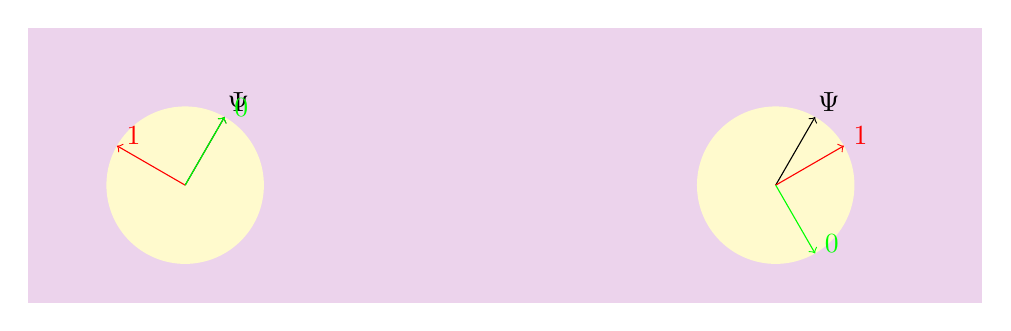
\begin{tikzpicture}%
\definecolor{lila}{RGB}{236,211,236}
\definecolor{lemonchiffon}{RGB}{255,250,205}
\fill[color=lila] (-7,-6.5) rectangle +(\the\textwidth,3.5);%vlak van tekening

\begin{scope}[xshift=-9.cm, yshift=-5cm]%base B
\def\baseangle{60}
\fill[color=lemonchiffon] (4,0) circle (1cm);
\draw [->] (4,0) -- +(60:1cm) node [label={[xshift=5pt, yshift=-5pt]$\ket{\Psi}$}]{};
\draw [red, ->] (4,0) -- +(90+\baseangle:1cm) node [label={[right]$\ket{1}$}]{};
\draw [green, ->] (4,0) -- +( 0+\baseangle:1cm) node [label={[right]$\ket{0}$}]{};
\end{scope}

\begin{scope}[xshift=-1.5cm, yshift=-5cm]%base B
\def\baseangle{-60}
\fill[color=lemonchiffon] (4,0) circle (1cm);
\draw [->] (4,0) -- +(60:1cm) node [label={[xshift=5pt, yshift=-5pt]$\ket{\Psi}$}]{};
\draw [red, ->] (4,0) -- +(90+\baseangle:1cm) node [label={[right]$\ket{1}$}]{};
\draw [green, ->] (4,0) -- +( 0+\baseangle:1cm) node [label={[right]$\ket{0}$}]{};
\end{scope}

\end{tikzpicture}%

\begin{tikzpicture}%
\definecolor{lila}{RGB}{236,211,236}
\definecolor{lemonchiffon}{RGB}{255,250,205}
\fill[color=lila] (-7,-6.7) rectangle +(4.,3.5);%vlak van tekening
\begin{scope}[xshift=-5.cm, yshift=-5cm]%base B
\def\ojfrangle{-60}%rotated frame
\def\ojobangle{90}% object =black arrow

\node (O) at(0,0) {};
\fill[color=lemonchiffon] (O) circle (1cm);

\draw [black, ->] (O.center) -- +(\ojobangle:1cm) node (Psi) {};
\node at (\ojobangle:1.3cm) {$\ket{\Psi}$};

\draw [thick, red, ->]   (O.center) -- +(90+\ojfrangle:1cm) node (Ket1){};
\node [red] at (90+\ojfrangle:1.3cm) {$\ket{1}$};
\draw [thick, green, ->] (O.center) -- +( 0+\ojfrangle:1cm) node (Ket0){};
\node [green] at (0+\ojfrangle:1.3cm) {$\ket{0}$};
\draw [dotted] ($(O)!(Psi)!(Ket1)$) -- (Psi);;
\draw [dotted] ($(O)!(Psi)!(Ket0)$) -- (Psi);;
\draw [lightgray, thin]   (O.center) -- +(-90+\ojfrangle:1cm);
\draw [lightgray, thin]   (O.center) -- +(180+\ojfrangle:1cm);
\end{scope}
\node at(-5,-6.3) {Alice};
\end{tikzpicture}%

\end{document}